\documentclass[11pt]{report}

\usepackage{epsf,amsmath,amsfonts}
\usepackage{graphicx}

\setlength{\textwidth}{6.5in}
\setlength{\oddsidemargin}{0in}
\setlength{\evensidemargin}{0in}
\setlength{\textheight}{8.5in}
\setlength{\topmargin}{0in}

\begin{document}

\title{
Requirements and Design\\
Tensor Operators}
\author{MPAS Development Team}

\maketitle
\tableofcontents

%-----------------------------------------------------------------------

\chapter{Summary}

The computation of the stress tensor and the divergence of the stress tensor are required for turbulence closures and the sea-ice momentum equation.  These operations on an unstructured grid are significantly more complicated than on a quadrilateral grid.  Here we provide algorithms to compute the strain rate tensor, as a simplification from the full stress tensor.  Computation of the strain rate tensor is the difficult part, while the stress tensor equations are dependant on the choice of model equations.  The divergence of a tensor is also presented, as well as many analytic test cases to validate both operators.


%figure template
%\begin{figure}
%  \center{\includegraphics[width=14cm]{./Figure1.pdf}}
%  \caption{A graphical representation of the discrete boundary.}
%  \label{Figure1}
%\end{figure} 

%-----------------------------------------------------------------------

\chapter{Requirements}

\section{Requirement: strain rate tensor}
Date last modified: 2/12/2013 \\
Contributors: Mark Petersen \\

 Given a discrete horizontal velocity field on the edges of an unstructured C-grid, compute the strain rate tensor 
\begin{equation}
\dot{\epsilon}_{ij} = \frac{1}{2}\left(\frac{\partial u_i}{\partial x_j} 
                                     + \frac{\partial u_j}{\partial x_i}\right)
\end{equation}
at cell centers and vertices.  

For an analytic test function, the computed strain rate tensor must converge to the analytic solution as the grid is refined.  This must be tested on quad, hex, and variable resolution grids.

{\it comment by Todd:} Are there any order-of-accuracy and/or conservation requirements? {\it Mark: I'm not sure.}

\section{Requirement: divergence of a tensor}
Date last modified: 2/12/2013 \\
Contributors: Mark Petersen \\

Given a two-dimensional tensor, $\sigma$, at cell centers and vertices of an unstructured C-grid, compute $(\nabla\cdot\sigma)\cdot{\bf n}_e$, the normal component of the divergence of the tensor at an edge.

For an analytic test function, the computed divergence must converge to the analytic solution as the grid is refined.  This must be tested on quad, hex, and variable resolution grids.

{\it comment by Todd:} Are there any order-of-accuracy and/or conservation requirements? {\it Mark: I'm not sure.}


%-----------------------------------------------------------------------

\chapter{Algorithmic Formulations}

\section{Design Solution: Strain rate tensor, projection}
Date last modified: 2/12/2013 \\
Contributors: Mark Petersen \\

The strain rate tensor is an important operator for many applications.  In CICE, the stress tensor is computed from the strain rate tensor in each grid cell with a system of ODEs \cite[section 3.4]{CICE_manual_4.1}.  The computation of the stress tensor depends on the details of the model.  For example, they differ between viscous-plastic and elastic-viscous-plastic in CICE.  Computation of the strain rate tensor is a general operation, and can be placed in the operators subdirectory so it may be used by all mpas cores.

\subsection{Continuous strain rate tensor}

The strain rate tensor in Cartesian coordinates is
\begin{equation}
\dot{\epsilon}_{ij} = \frac{1}{2}\left(\frac{\partial u_i}{\partial x_j} 
                                     + \frac{\partial u_j}{\partial x_i}\right),
\end{equation}
where ${\bf u} = (u_1,u_2)$ is the velocity in orthogonal Cartesian coordinates $(x_1,x_2)$.  In an arbitrary reference frame the strain rate tensor may be written using the Jacobian operator $J=\nabla {\bf u}$ as
\begin{equation}
{\bf\dot{\epsilon}} = \nabla_s {\bf u} \equiv \frac{1}{2}\left(J + J^T\right),
\end{equation}
where $\nabla_s$ denotes the symmetric gradient operator.  The weak form of the symmetric gradient over a control surface $A$  is
\begin{equation}
\label{weak strain rate tensor}
\nabla_s {\bf u}
= \lim_{A\rightarrow(x,y)} \frac{1}{\tilde{A}} 
\int_{\partial A}\frac{1}{2}\left( 
  {\bf n}\otimes{\bf u} 
+ {\bf u}\otimes{\bf n}\right)dl
\end{equation}
where $\tilde{A} = \int_A dA$ is the area, $dl$ is an increment along the boundary $\partial A$, and ${\bf n}$ is a unit vector normal to the boundary \cite[equation 22]{Ringler06unpub}.  {\it Mark: I need to find a published reference for (\ref{weak strain rate tensor})}  The symbol $\otimes$ is the tensor product, which is the same as an outer product for two vectors.  In two-dimensional Cartesian space, ${\bf n}$ and ${\bf u}$ are both 2x1 vectors, and 
\begin{equation}
{\bf n}\otimes{\bf u} 
= \left( \begin{array}{c} n_1 \\ n_2 \end{array}   \right)
  \left( \begin{array}{cc} u_1 &  u_2 \end{array} \right)
= \left( \begin{array}{cc} n_1 u_1 & n_1 u_2 \\  n_2 u_1 & n_2 u_2 \end{array}   \right).
\end{equation}

\begin{figure}[htbp]
 \center
 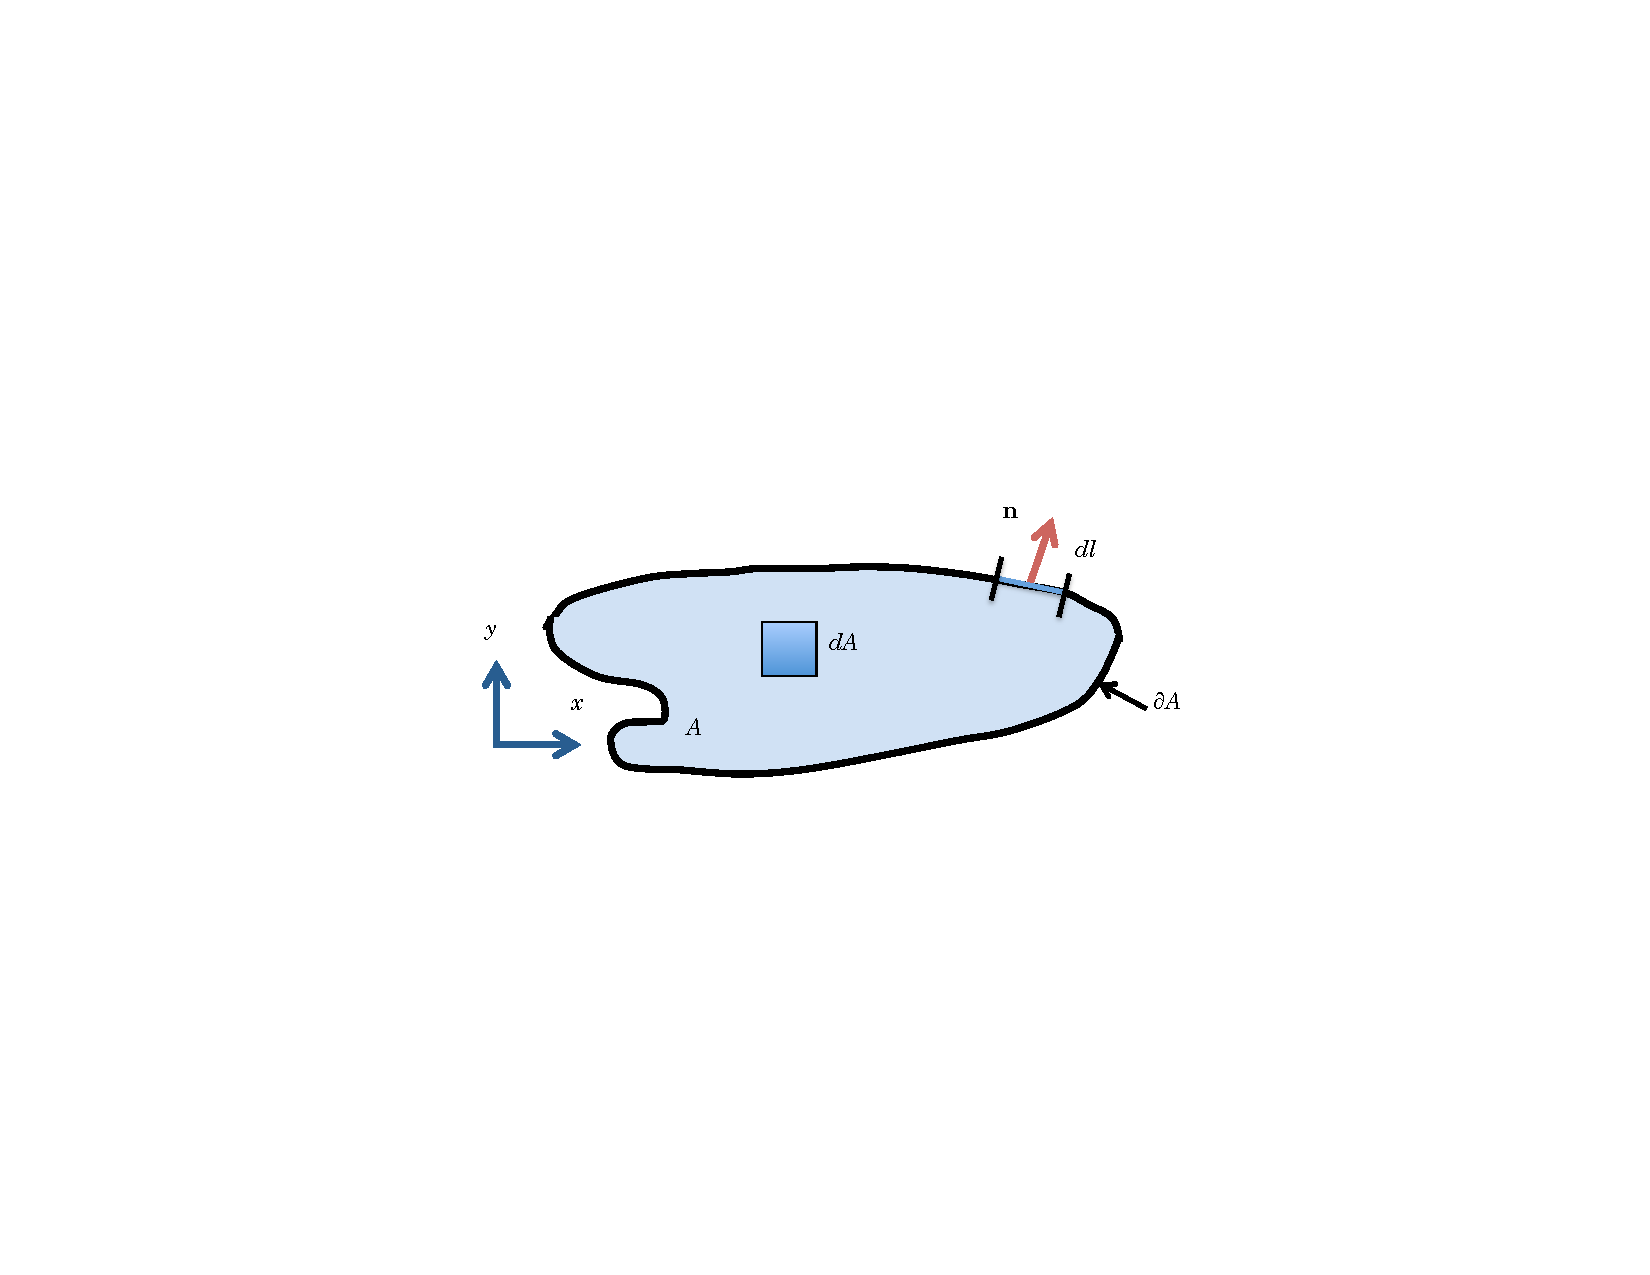
\includegraphics[trim=3.2in 3.2in 3.0in 3.5in, clip=true, scale=0.8]{f/A_surface.pdf}
 \caption{Two-dimensional surface $A$.}
 \label{fig:2D domain}
\end{figure}

\subsection{Discrete 2D strain rate tensor at cell centers}

Here we compute the strain rate tensor at a cell center ${\bf x}_i$ based on the normal and tangential velocities, ${\bf u}_e$ and ${\bf v}_e$, at the edges of that cell (Figure \ref{fig:edge vectors}).  The total velocity at edge $e$ is $({\bf u}_e + {\bf v}_e)$.  Discretizing the weak form (\ref{weak strain rate tensor}), the strain rate tensor at cell $i$ is
\begin{equation}
\label{cell strain rate tensor}
\left[\nabla_s {\bf u} \right]_i
= 
\frac{1}{A_i} 
\sum_{e\in EC(i)}{\frac{1}{2}\left( 
  {\bf n}_e\otimes\left({\bf u}_e +{\bf v}_e \right)
+ \left({\bf u}_e +{\bf v}_e \right)\otimes{\bf n}_e\right)l_e },
\end{equation}
where $A_i$ is the area of cell $i$, $l_e$ is the length of edge $e$, and ${\bf n}_e$ is the unit vector normal to edge $e$, and $EC(i)$ is the set of edges that bound cell $i$.

In order to proceed, we must choose a coordinate system to conduct these computations.  The MPAS framework includes an \verb|angleEdge| value for each edge, where \verb|angleEdge=0| when ${\bf n}_e$ points eastward, \verb|angleEdge|$=\pi/2$ when ${\bf n}_e$ points northward, etc.  

{\it comment by Todd:} How robust is this near the pole?  i.e. how far does the edge have to be away from the pole for the computation to be correct? {\it Mark:} That is something to test.  See Chapter on testing.

\begin{figure}[htbp]
 \center
 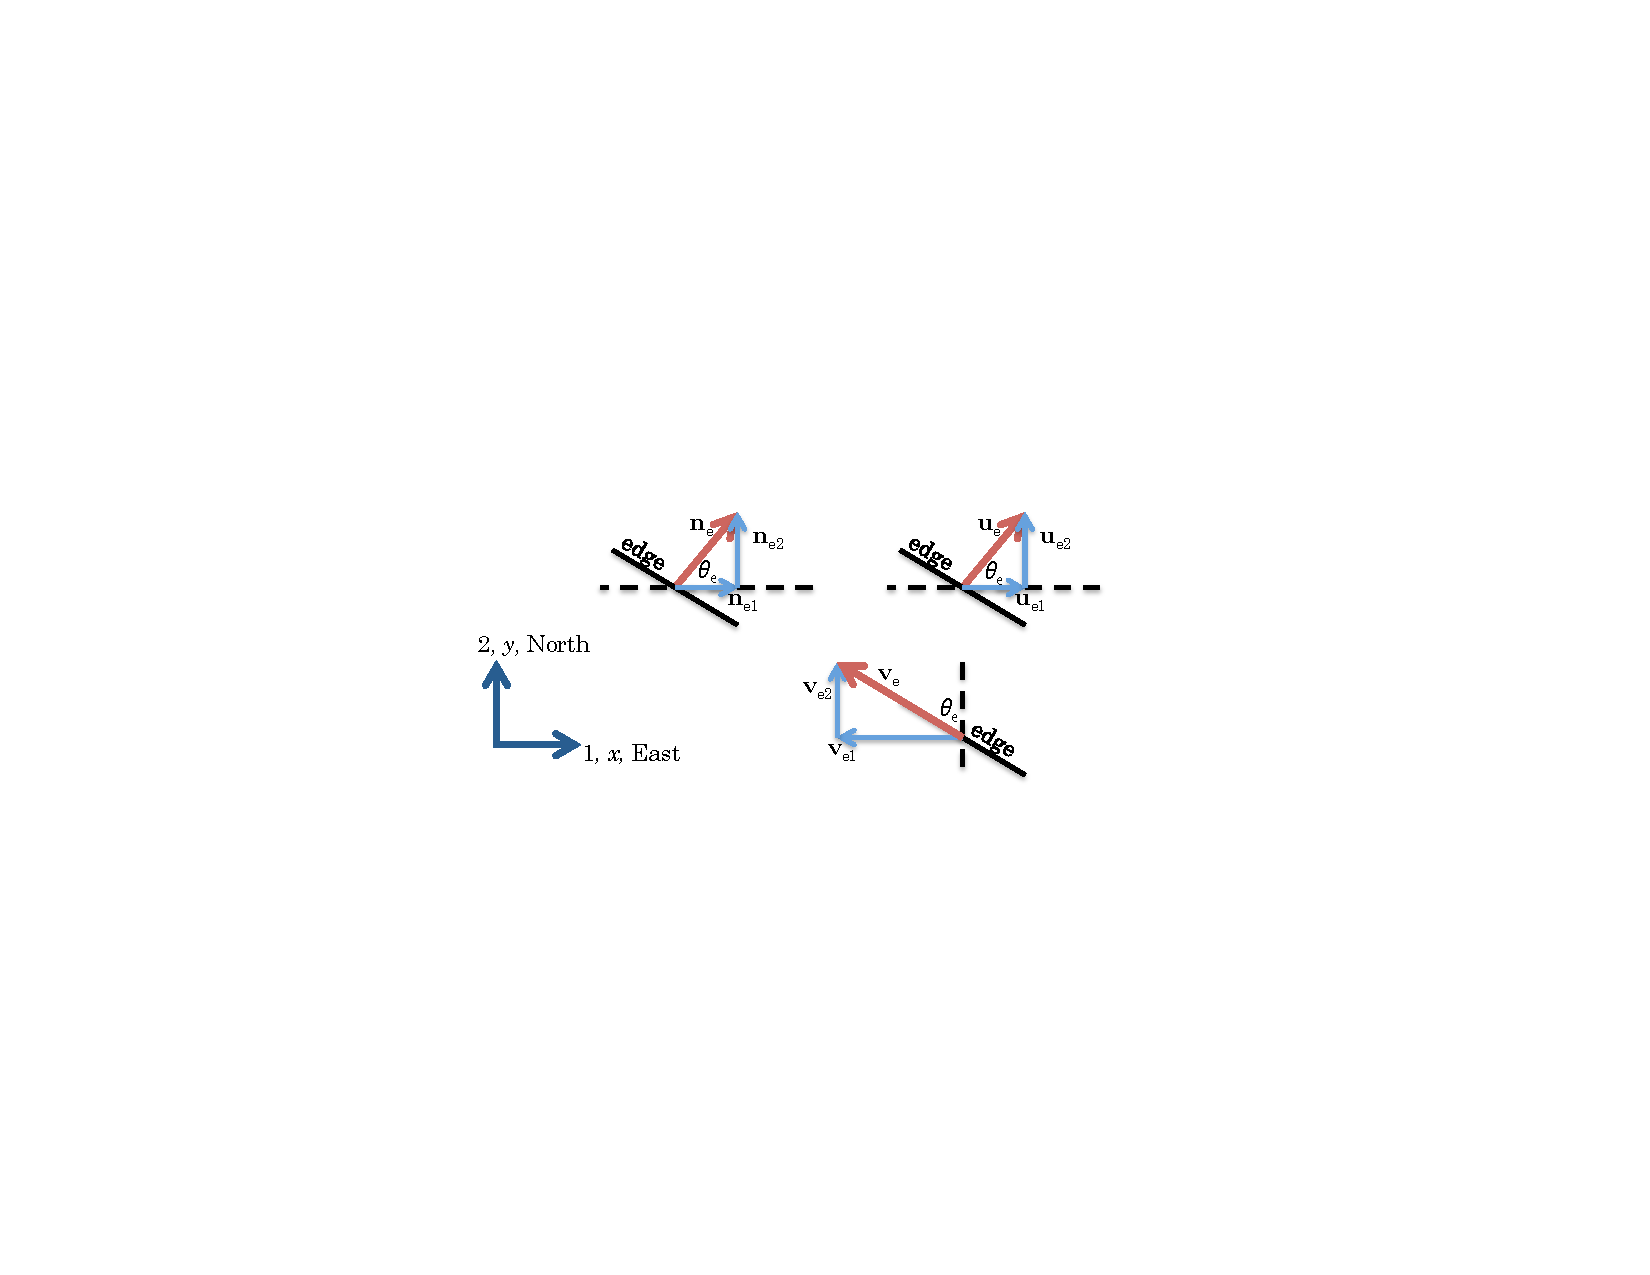
\includegraphics[trim=3.2in 3.2in 3.0in 3.2in, clip=true, scale=1.0]{f/u_v_coord_e.pdf}
 \caption{Decomposition of vectors at a cell edge: ${\bf n}_e$ is the unit vector normal to an edge; ${\bf u}_e$ is the normal velocity; ${\bf v}_e$ is the tangential velocity; and $\theta_e$ is the edge angle.}
 \label{fig:edge vectors}
\end{figure}

Vectors may be decomposed into local Cartesian components as
\begin{eqnarray}
&&{\bf n}_e = \left( \begin{array}{c} n_{e1} \\ n_{e2} \end{array} \right)
  = \left( \begin{array}{c} \cos{\theta_{e}} \\ \sin{\theta_{e}} \end{array} \right)\\
\label{u_e}
&&{\bf u}_e = \left( \begin{array}{c} u_{e1} \\ u_{e2} \end{array} \right)
  = \left( \begin{array}{c} u_e \cos{\theta_{e}} \\ u_e \sin{\theta_{e}} \end{array} \right)\\
\label{v_e}
&&{\bf v}_e = \left( \begin{array}{c} v_{e1} \\ v_{e2} \end{array} \right)
  = \left( \begin{array}{r} -v_e \sin{\theta_{e}} \\ v_e \cos{\theta_{e}} \end{array} \right)
\end{eqnarray}
where $u_e = |{\bf u}_e|$ and $v_e = |{\bf v}_e|$ are the velocity magnitudes stored in the model variables \verb|u| and \verb|v|.  The formulation of components in (\ref{v_e}) is due to the convention that ${\bf v}_e$ is 90 degrees counter-clockwise from ${\bf u}_e$, as shown in Figure \ref{fig:edge vectors}.  Proceeding from (\ref{cell strain rate tensor}), the strain rate tensor at a cell center may be computed as 
\begin{eqnarray}
&\left[\nabla_s {\bf u} \right]_i
= \displaystyle
\frac{1}{A_i} 
\sum_{e\in EC(i)} 
\left( \begin{array}{cc} (u_{e1} + v_{e1})n_{e1}  
               & \frac{1}{2}((u_{e1} + v_{e1})n_{e2} + (u_{e2} + v_{e2})n_{e1}) \\ 
                 (sym)  &
                       (u_{e2} + v_{e2})n_{e2} \end{array} \right) l_e\\
&=\displaystyle\frac{1}{A_i} \sum_{e\in EC(i)} 
\left( \begin{array}{cc} u_e \cos^2\theta_e - v_e \cos{\theta_e} \sin{\theta_e} 
 & u_e \cos{\theta_e} \sin{\theta_e} + \frac{1}{2}v_e\left(\cos^2\theta_e - \sin^2\theta_e\right)\\
   (sym)
 &                     u_e \sin^2\theta_e + v_e \cos{\theta_e} \sin{\theta_e} \end{array} \right)l_e
\end{eqnarray}
where $(sym)$ indicates that $\dot{\epsilon}_{21}=\dot{\epsilon}_{12}$ on this symmetric matrix.


\subsection{Discrete 2D strain rate tensor at vertices}

The strain rate computation at vertices is similar to that for cells, except that the control area is now a dual-mesh cell centered on vertex at ${\bf x}_v$, bounded by lines of length $d_e$ connecting primal-mesh cell centers \cite[figure 1]{Ringler_ea10jcp}.  The normal vector to an edge on the dual-mesh is
\begin{eqnarray}
&&\tilde{\bf n}_e = \left( \begin{array}{c} \tilde{n}_{e1} \\ \tilde{n}_{e2} \end{array} \right)
  = \left( \begin{array}{r} \sin{\theta_{e}} \\ -\cos{\theta_{e}} \end{array} \right),
\end{eqnarray}
so that $\tilde{\bf n}_e$ is rotated clockwise from ${\bf n}_e$ by 90 degrees.  The projections of ${\bf u}_e$ and ${\bf v}_e$ remain the same as in (\ref{u_e}--\ref{v_e}).  The strain rate tensor at a vertex is then
\begin{eqnarray}
&\left[\nabla_s {\bf u} \right]_v
= \displaystyle \frac{1}{A_v} 
\sum_{e\in EV(v)}{\frac{1}{2}\left( 
  \tilde{\bf n}_e\otimes\left({\bf u}_e +{\bf v}_e \right)
+ \left({\bf u}_e +{\bf v}_e \right)\otimes\tilde{\bf n}_e\right)l_e },
\label{vertex strain rate tensor2}
\\
& = \displaystyle
\frac{1}{A_v} 
\sum_{e\in EV(v)} 
\left( \begin{array}{cc} (u_{e1} + v_{e1})\tilde{n}_{e1}  
               & \frac{1}{2}((u_{e1} + v_{e1})\tilde{n}_{e2} + (u_{e2} + v_{e2})\tilde{n}_{e1}) \\ 
                 (sym)  &
                       (u_{e2} + v_{e2})\tilde{n}_{e2} \end{array} \right) l_e
\\
&=\displaystyle\frac{1}{A_v} \sum_{e\in EV(v)} 
\left( \begin{array}{cc} -v_e \sin^2\theta_e + u_e \cos{\theta_e} \sin{\theta_e} 
 & v_e \cos{\theta_e} \sin{\theta_e} + \frac{1}{2}u_e\left(\sin^2\theta_e - \cos^2\theta_e\right)\\
   (sym)
 &                     -v_e \cos^2\theta_e - u_e \cos{\theta_e} \sin{\theta_e} \end{array} \right)l_e
\end{eqnarray}

\subsection{Discrete 3D strain rate tensor at cell centers}

Here we present the full three-dimensional calculation for a strain rate tensor.  This version avoids the use of $\theta_e$, the \verb|angleEdge| variable, altogether, and so does not have any issues near the pole.  However, this is at the expense of going from a 2x2 symmetric tensor to a 3x3 symmetric tensor.  It is also not clear how to generalize the 2D tensor operations in the CICE dynamics \cite[section 3.4]{CICE_manual_4.1}.  

Beginning with (\ref{cell strain rate tensor2})
\begin{equation}
\label{cell strain rate tensor2}
\left[\nabla_s {\bf u} \right]_i
= 
\frac{1}{A_i} 
\sum_{e\in EC(i)}{\frac{1}{2}\left( 
  {\bf n}_e\otimes\left({\bf u}_e +{\bf v}_e \right)
+ \left({\bf u}_e +{\bf v}_e \right)\otimes{\bf n}_e\right)l_e },
\end{equation}
we rewrite the normal and tangential velocities in terms of a scalar coefficient and a unit vector,
\begin{eqnarray}
{\bf u}_e = u_e {\bf n}_e, 
  && {\bf n}_e = \frac{{\bf x}_{i2}-{\bf x}_{i1}}{\left||{\bf x}_{i2}-{\bf x}_{i1}\right||}
  = \frac{1}{d_e} \sum_{i\in CE(e)}n_{e,i}{\bf x}_{i} 
\\
{\bf v}_e = v_e \tilde{\bf n}_e, 
  && \tilde{\bf n}_e = \frac{{\bf x}_{v2}-{\bf x}_{v1}}{\left||{\bf x}_{v2}-{\bf x}_{v1}\right||}
  = \frac{1}{d_v} \sum_{v\in VE(e)}n_{e,i}{\bf x}_{v}?
\end{eqnarray}
I have not settled on the best notation yet, but ${\bf n}_e$ is the unit vector normal to the edge, and $\tilde{\bf n}_e $ is the unit vector tangent to the edge, pointing in the same direction as ${\bf v}_e$.  Continuing from (\ref{cell strain rate tensor2}), 
\begin{equation}
\label{cell strain rate tensor3}
\left[\nabla_s {\bf u} \right]_i
= 
\frac{1}{A_i} 
\sum_{e\in EC(i)}{\frac{1}{2}\left( 
 2u_e{\bf n}_e\otimes{\bf n}_e
+ v_e{\bf n}_e\otimes\tilde{\bf n}_e
+ v_e\tilde{\bf n}_e\otimes{\bf n}_e
\right)l_e }.
\end{equation}
The unit vectors ${\bf n}_e$ and $\tilde{\bf n}_e$ are 3-vectors in $(x,y,z)$ space, making the tensor products 3x3 tensors.


\subsection{Discrete 3D strain rate tensor at vertices}

Beginning with (\ref{vertex strain rate tensor3}),
\begin{eqnarray}
\label{vertex strain rate tensor3}
\left[\nabla_s {\bf u} \right]_v
&=& \displaystyle \frac{1}{A_v} 
\sum_{e\in EV(v)}{\frac{1}{2}\left( 
  \tilde{\bf n}_e\otimes\left({\bf u}_e +{\bf v}_e \right)
+ \left({\bf u}_e +{\bf v}_e \right)\otimes\tilde{\bf n}_e\right)l_e },
\\
&=& \displaystyle \frac{1}{A_v} 
\sum_{e\in EV(v)}{\frac{1}{2}\left( 
 2v_e\tilde{\bf n}_e\otimes\tilde{\bf n}_e
+ u_e{\bf n}_e\otimes\tilde{\bf n}_e
+ u_e\tilde{\bf n}_e\otimes{\bf n}_e
\right)l_e },
\end{eqnarray}
so that a 3x3 strain rate tensor is computed for each vertex.

\newpage
\section{Design Solution: divergence of a tensor}
Date last modified: 2/12/2013 \\
Contributors: Mark Petersen \\

\subsection{2D divergence of a tensor}

In two-dimensional Cartesian coordinates, the component of the divergence of a tensor $\sigma$ in the direction of a unit vector ${\bf n}$ is 
\begin{eqnarray}
\left(\nabla\cdot\sigma\right)\cdot{\bf n}
 &=& \left(
\left(\begin{array}{cc} \partial_1 &  \partial_2 \end{array} \right)
\left(\begin{array}{cc} \sigma_{11} &  \sigma_{12} \\
                        \sigma_{21} &  \sigma_{22} \end{array} \right)
\right)\cdot{\bf n}\\
 &=& 
\left(\begin{array}{c} \sigma_{11,1} + \sigma_{21,2} \\
                        \sigma_{12,1} + \sigma_{22,2} \end{array}
\right)\cdot\left(\begin{array}{c} n_1 \\ n_2 \end{array} \right)\\
\label{sigma1}
 &=& 
  \left( \sigma_{11,1} + \sigma_{21,2}\right) n_1
+ \left( \sigma_{12,1} + \sigma_{22,2}\right) n_2
\end{eqnarray}
The diagonal terms of the stress tensor are the normal components, and represent stress due to compressive (and expansive) forces; $\sigma_{11}$ is compression in 1 direction, and $\sigma_{22}$ is compression in the 2 direction.  The off-diagonal terms are due to shear in the 1 and 2 directions.  However, pure compression or pure shear not aligned with the 1 or 2 directions will result in components in both diagonal and off-diagonal elements of the stress tensor.

In most cases we are interested in projecting the divergence of a tensor onto ${\bf n}_e$, the normal to a cell edge.  For example, the momentum equation for sea-ice requires this term when computing the tendencies of $u_e$ \cite[section 3.4]{CICE_manual_4.1}.  It is therefore convenient to arrange a local Cartesian coordinate system where the 1-direction is aligned with ${\bf n}_e$ (i.e. pointing from one cell center to the other) and the 2-direction is aligned with $\tilde{\bf n}_e$ (i.e. pointing from one vertex to the other).  This is possible because on a Voronoi tesselation grid, the line joining cell centers across a cell edge is always orthogonal to that cell edge.  A tensor may be rotated through an angle $\theta$ into a new coordinate system using rotation matrices as
\begin{eqnarray}
\label{rotate sigma 2D}
\tilde{\sigma} &=& R_\theta \sigma R_\theta^*,\\
&=& 
\left(\begin{array}{cc} \cos{\theta}& -\sin{\theta} \\
                        \sin{\theta}&  \cos{\theta} 
 \end{array} \right)
\left(\begin{array}{cc} \sigma_{11} & \sigma_{12} \\
                        \sigma_{21} & \sigma_{22} 
 \end{array} \right)
\left(\begin{array}{cc} \cos{\theta}&  \sin{\theta} \\
                       -\sin{\theta}&  \cos{\theta} 
 \end{array} \right) \\
&=& 
\left(\begin{array}{cc} \sigma_{11}\cos{\theta} - \sigma_{21}\sin{\theta} &
                        \sigma_{12}\cos{\theta} - \sigma_{22}\sin{\theta} \\
                        \sigma_{11}\sin{\theta} + \sigma_{21}\cos{\theta} &
                        \sigma_{12}\sin{\theta} + \sigma_{22}\cos{\theta} 
 \end{array} \right)
\left(\begin{array}{cc} \cos{\theta}&  \sin{\theta} \\
                       -\sin{\theta}&  \cos{\theta} 
 \end{array} \right) \\
&=& 
\left(\begin{array}{cc} 
  \sigma_{11}\cos^2{\theta} - 2\sigma_{12}\cos{\theta}\sin{\theta} + \sigma_{22}\sin^2{\theta} &
  (\sigma_{11}- \sigma_{22})\cos{\theta}\sin{\theta} + \sigma_{12}\left(\cos^2{\theta} - \sin^2{\theta} \right)  \\
(sym) &
  \sigma_{11}\sin^2{\theta} + 2\sigma_{12}\cos{\theta}\sin{\theta} + \sigma_{22}\cos^2{\theta} 
 \end{array} \right)
\end{eqnarray}
where $*$ is the transpose.  In the rotated coordinate system, the divergence of a tensor simplifies to
\begin{eqnarray}
\left[(\nabla\cdot\sigma)\cdot{\bf n}_e\right]_e =   \tilde\sigma_{11,1} + \tilde\sigma_{21,2}
\end{eqnarray}
and the standard strong form of the discrete derivative \cite[equation 22]{Ringler_ea10jcp} may be used,
\begin{eqnarray}
\label{discrete div1}
\left[(\nabla\cdot\sigma)\cdot{\bf n}_e\right]_e
 &=& \frac{1}{d_e} \sum_{i\in CE(e)}-n_{e,i}\left[\tilde\sigma_{11}\right]_i
   + \frac{1}{l_e} \sum_{v\in VE(e)}-t_{e,v}\left[\tilde\sigma_{12}\right]_v
\\
 &=& \frac{1}{d_e} \sum_{i\in CE(e)}-n_{e,i}\left(
\left[\sigma_{11}\right]_i\cos^2{\theta_e} - 2\left[\sigma_{12}\right]_i\cos{\theta_e}\sin{\theta_e} + \left[\sigma_{22}\right]_i\sin^2{\theta_e}
\right) \nonumber \\
 &&+ \frac{1}{l_e} \sum_{v\in VE(e)}-t_{e,v}\left(
  (\left[\sigma_{11}\right]_v- \left[\sigma_{22}\right]_v)\cos{\theta_e}\sin{\theta_e} + \left[\sigma_{12}\right]_v\left(\cos^2{\theta_e} - \sin^2{\theta_e} \right)  
\right).
\label{discrete div2}
\end{eqnarray}

{\it Todd:} It seems to me that you are done at \ref{sigma1}. The (div cot sigma) dot n is a scalar. As long as you have measured everything in the same coordinate system, there should be no need to rotate anything. simply compute \ref{sigma1} with n in the direction(s) of interest.

{\it Response, Mark:} I only know the sigma tensor at cell centers and vertices.  How could I compute \ref{sigma1} for any n in the 1,2 reference frame using strong derivatives, as in \ref{discrete div1}?  The only solution I can think of is to rotate the tensor so that the directions to take derivatives aligns parallel and perpendicular to the local edge.  This then conforms with our standard methods of finite differences. 

\subsection{3D divergence of a tensor}

The general form required is the divergence of a tensor normal to edge $e$,
\begin{equation}
(\nabla\cdot\sigma)\cdot{\bf n}_e,
\end{equation}
is coordinate free, and may be computed in three dimensions.  The difficulty is that we only have information at the cell centers and vertices, and so must take strong derivatives in those directions.  This is the same issue that required rotating the tensor in 2D in (\ref{rotate sigma 2D}).  This time we rotate in 3D,
\begin{eqnarray}
\tilde{\sigma}_{i,e} &=& R_e\sigma_i R_e^*,
\\
\tilde{\sigma}_{v,e} &=& R_e\sigma_v R_e^*,
\\
R_e &=& \left[ 
\begin{array}{ccc}
{\bf n}_e & \tilde{\bf n}_e & {\bf n}_e\times\tilde{\bf n}_e  
\end{array}
\right]
\\
\left[(\nabla\cdot\sigma)\cdot{\bf n}_e\right]_e &=& \tilde\sigma_{11,1} + \tilde\sigma_{21,2},
\\
 &=& \frac{1}{d_e} \sum_{i\in CE(e)}-n_{e,i}\left[\tilde\sigma_{11}\right]_{i,e}
   + \frac{1}{l_e} \sum_{v\in VE(e)}-t_{e,v}\left[\tilde\sigma_{12}\right]_{v,e}
\end{eqnarray}
where the 1-direction points from cell to cell with ${\bf n}_e$, the 2-direction points from vertex to vertex with $\tilde{\bf n}_e$, and the 3-direction is perpendicular to those directions, using ${\bf n}_e\times\tilde{\bf n}_e$.  The rotation matrix $R_e$ is simply composed of those three vectors, and the operation $R_e\sigma_i R_e^*$ rotates the original tensor in an $(x,y,z)$ reference frame to the new reference frame.  All components of the rotated stress tensor with a 3 index ($\tilde\sigma_{13}$, $\tilde\sigma_{23}$, $\tilde\sigma_{33}$, etc.) should be small because velocities are tangent to the earth, but may not be exactly zero due to the curvature of the earth from one cell to the next.  For domains in the $x-y$ plane, ${\bf n}_e\times\tilde{\bf n}_e=(0,0,1)$ for all edges, and all elements of $\tilde\sigma_{ij}$ with an index value of three will be exactly zero.


%-----------------------------------------------------------------------

\chapter{Design and Implementation}

\section{Implementation: 2D strain rate tensor}
Date last modified: 2/12/2013 \\
Contributors: Mark Petersen \\


\begin{verbatim}
subroutine mpas_strain_rate(grid, u,v, strainRateCell, strainRateVertex)!{{{

...

strainRateCell = 0.0
strainRateVertex = 0.0

do iEdge=1,nEdges
   vertex1 = verticesOnEdge(1,iEdge)
   vertex2 = verticesOnEdge(2,iEdge)

   cell1 = cellsOnEdge(1,iEdge)
   cell2 = cellsOnEdge(2,iEdge)

   invAreaTri1 = 1.0 / areaTriangle(vertex1)
   invAreaTri2 = 1.0 / areaTriangle(vertex2)

   invAreaCell1 = 1.0 / max(areaCell(cell1), 1.0)
   invAreaCell2 = 1.0 / max(areaCell(cell2), 1.0)

   cos_pwr1 = cos(angleEdge(iEdge))
   cos_pwr2 = cos_pwr1**2
   sin_pwr1 = sin(angleEdge(iEdge))
   sin_pwr2 = sin_pwr1**2
   cossin = cos_pwr1*sin_pwr1

   do k=1,nVertLevels

      ! strain rate tensor at cell center
      eps11 = u(k,iEdge)*cos_pwr2   - v(k,iEdge)*cossin
      eps22 = u(k,iEdge)*sin_pwr2   + v(k,iEdge)*cossin
      eps12 = u(k,iEdge)*cossin + v(k,iEdge)*0.5*(cos_pwr2-sin_pwr2)

      ! index 1, 2, and 3 is for 11, 22, and 12 
      strainRateCell(1,k,cell1) = strainRateCell(1,k,cell1) &
                                  + eps11*invAreaCell1 * dvEdge(iEdge)
      strainRateCell(1,k,cell2) = strainRateCell(1,k,cell2) &
                                  - eps11*invAreaCell2 * dvEdge(iEdge)
      strainRateCell(2,k,cell1) = strainRateCell(2,k,cell1) &
                                  + eps22*invAreaCell1 * dvEdge(iEdge)
      strainRateCell(2,k,cell2) = strainRateCell(2,k,cell2) &
                                  - eps22*invAreaCell2 * dvEdge(iEdge)
      strainRateCell(3,k,cell1) = strainRateCell(3,k,cell1) &
                                  + eps12*invAreaCell1 * dvEdge(iEdge)
      strainRateCell(3,k,cell2) = strainRateCell(3,k,cell2) &
                                  - eps12*invAreaCell2 * dvEdge(iEdge)

      ! strain rate tensor at vertex
      eps11 = -v(k,iEdge)*sin_pwr2   + u(k,iEdge)*cossin
      eps22 = -v(k,iEdge)*cos_pwr2   - u(k,iEdge)*cossin
      eps12 =  v(k,iEdge)*cossin - u(k,iEdge)*0.5*(cos_pwr2-sin_pwr2)

      strainRateVertex(1,k,vertex1) = strainRateVertex(1,k,vertex1) &
                                  - eps11*invAreaTri1* dcEdge(iEdge)
      strainRateVertex(1,k,vertex2) = strainRateVertex(1,k,vertex2) &
                                  + eps11*invAreaTri2* dcEdge(iEdge)
      strainRateVertex(2,k,vertex1) = strainRateVertex(2,k,vertex1) &
                                  - eps22*invAreaTri1* dcEdge(iEdge)
      strainRateVertex(2,k,vertex2) = strainRateVertex(2,k,vertex2) &
                                  + eps22*invAreaTri2* dcEdge(iEdge)
      strainRateVertex(3,k,vertex1) = strainRateVertex(3,k,vertex1) &
                                  - eps12*invAreaTri1* dcEdge(iEdge)
      strainRateVertex(3,k,vertex2) = strainRateVertex(3,k,vertex2) &
                                  + eps12*invAreaTri2* dcEdge(iEdge)

   end do
end do
\end{verbatim}
\newpage
{\it Todd:} Is it worth the 25\% cost in memory to declare this 2,2 and then have something that can be used directly in matrix operations (and rotations and dot products and cross products ?)? I think that the 1,2,3 storage will lead to a proliferation of code in order to keep track of xx,yy,xy as a vector.

{\it Response, Mark:} I chose to store three, rather than include a redundant forth, because I don't see the need for general array operations on this 2x2 matrix.  The divergence is computed with \ref{discrete div2}, where the rotation-matrix multiplies are pre-computed.  In the CICE formulation \cite[section 3.4, equation 52]{CICE_manual_4.1}, $\sigma_{12}$ is used in the terms of an ODE, not in a matrix multiply.
   

\newpage
\section{Implementation: 2D divergence of a tensor}
Date last modified: 2/12/2013 \\
Contributors: Mark Petersen \\

\begin{verbatim}
subroutine mpas_div_tensor(grid, tensorCell, tensorVertex, divTensor)!{{{

...

do iEdge=1,nEdgesSolve
   vertex1 = verticesOnEdge(1,iEdge)
   vertex2 = verticesOnEdge(2,iEdge)

   cell1 = cellsOnEdge(1,iEdge)
   cell2 = cellsOnEdge(2,iEdge)

   cos_pwr1 = cos(angleEdge(iEdge))
   cos_pwr2 = cos_pwr1**2
   sin_pwr1 = sin(angleEdge(iEdge))
   sin_pwr2 = sin_pwr1**2
   cossin = cos_pwr1*sin_pwr1

   invdcEdge = 1.0 / dcEdge(iEdge)
   invdvEdge = 1.0 / dvEdge(iEdge)

   do k=1,maxLevelEdgeTop(iEdge)
      divTensor(k,iEdge) = &
         edgeMask(k,iEdge) * invdcEdge &
         * (        cos_pwr2  *tensorCell(1,k,cell2) &
              - 2.0*cossin*tensorCell(3,k,cell2) &
                  + sin_pwr2  *tensorCell(2,k,cell2) &
            -(      cos_pwr2  *tensorCell(1,k,cell1) &
              - 2.0*cossin*tensorCell(3,k,cell1) &
                  + sin_pwr2  *tensorCell(2,k,cell1)) ) &
       + edgeMask(k,iEdge) * invdvEdge &
         * (   (cos_pwr2-sin_pwr2)*tensorVertex(3,k,vertex2) &
              + cossin*(   tensorVertex(1,k,vertex2) &
                         - tensorVertex(2,k,vertex2)) &
            -( (cos_pwr2-sin_pwr2)*tensorVertex(3,k,vertex1) &
              + cossin*(   tensorVertex(1,k,vertex1) &
                         - tensorVertex(2,k,vertex1))))
   end do

end do
\end{verbatim}

%-----------------------------------------------------------------------

\chapter{Testing and Validation}

\section{Testing functions for strain rate and its divergence on a plane}
Date last modified: 2/12/2013 \\
Contributors: Mark Petersen \\

The following analytic test cases may be used to test the tensor operators on any two-dimension Cartesian domain, including quads, hexes, and variable resolution meshs.  There are presently no test cases for a sphere.  All cases are implemented in the subroutine \verb|mpas_test_tensor|.  It is clear that some later test cases are a superset of earlier ones.  For example, the linear case is the power function with $n=1$.  But the earlier simple cases are instructional and useful for debugging, and so are included here and in the code.

The constant coefficients $c_n$ and $c_s$ are for the normal and shear components of the strain, respectively.  When velocities are aligned with an axis, like in cases \ref{linear_x}, \ref{linear_y}, \ref{power_x}, and \ref{power_y}, the normal strain appears on the diagonals of the strain rate tensor, and the shear appears on the off-diagonals.  However, for arbitrary rotations, both components appear in all the elements of the strain rate tensor.

\subsection{Linear in x\label{linear_x}}
\begin{eqnarray}
{\bf u}(x,y) &=& \left( \begin{array}{c} c_n \\ c_s \end{array}   \right)x \\
\nabla{\bf u}^* &=& \left( \begin{array}{c} \partial_x \\ \partial_y \end{array}   \right) \left( \begin{array}{cc} c_nx & c_sx \end{array}   \right)
 =  \left( \begin{array}{cc} c_n & c_s \\ 0 & 0 \end{array}   \right) \\
\nabla_s{\bf u}^* &=&  \left( \begin{array}{cc} c_n & \frac{1}{2}c_s \\ \frac{1}{2}c_s & 0 \end{array}   \right) \\
\nabla\cdot\left(\nabla_s{\bf u}\right) &=&  \left( \begin{array}{cc} 0 & 0 \end{array}   \right)
\end{eqnarray}

\subsection{Linear in y\label{linear_y}}
\begin{eqnarray}
{\bf u}(x,y) &=& \left( \begin{array}{c} -c_s \\ c_n \end{array}   \right)y \\
\nabla{\bf u}^* &=& \left( \begin{array}{c} \partial_x \\ \partial_y \end{array}   \right) \left( \begin{array}{cc} -c_sy & c_ny \end{array}   \right)
 =  \left( \begin{array}{cc}  0 & 0 \\ -c_s & c_n  \end{array}   \right) \\
\nabla_s{\bf u}^* &=&  \left( \begin{array}{cc} 0 & -\frac{1}{2}c_s \\ -\frac{1}{2}c_s & c_n \end{array}   \right) \\
\nabla\cdot\left(\nabla_s{\bf u}\right) &=&  \left( \begin{array}{cc} 0 & 0 \end{array}   \right)
\end{eqnarray}

\subsection{Linear, rotated about an arbitrary angle $\theta_r$\label{linear_rotation}}
\begin{eqnarray}
{\bf u}(r,\theta;\theta_r) &=& r\cos{(\theta-\theta_r)} R_{\theta_r} \left( \begin{array}{c} c_n \\ c_s \end{array}   \right) = f{\bf g}
\end{eqnarray}
where 
\begin{eqnarray}
\label{def f}
f(r,\theta;\theta_r)&\equiv& r\cos{(\theta-\theta_r)},\\
\label{def g}
{\bf g}(\theta_r) &\equiv& R_{\theta_r} \left( \begin{array}{c} c_n \\ c_s \end{array}   \right) \\
&=& \left(\begin{array}{cc} \cos{\theta_r}& -\sin{\theta_r} \\
                          \sin{\theta_r}&  \cos{\theta_r}   \end{array}\right)
 \left( \begin{array}{c} c_n \\ c_s \end{array}   \right)\\
&=& \left(\begin{array}{c} c_n\cos{\theta_r} -c_s\sin{\theta_r} \\
                          c_n\sin{\theta_r} +  c_s \cos{\theta_r}   \end{array}\right)
\end{eqnarray}
Note that when $\theta_r=0$ this simplifies to case \ref{linear_x} and when $\theta_r=\pi/2$ this simplifies to case \ref{linear_y}.  Recall the trig identity
\begin{equation}
\cos{(a-b)} = \cos{a}\cos{b} + \sin{a}\sin{b}
\end{equation}
so that 
\begin{eqnarray}
f&\equiv& r\cos{(\theta-\theta_r)}\\
 &=& r\cos{\theta}\cos{\theta_r} + r\sin{\theta}\sin{\theta_r}\\
 &=& x\cos{\theta_r} + y\sin{\theta_r}.
\end{eqnarray}
Finally, the operators of interest for this test case are
\begin{eqnarray}
\nabla{\bf u}^* &=& \left( \nabla f \right) {\bf g}^* 
 = \left( \begin{array}{c} \cos{\theta_r} \\ \sin{\theta_r} \end{array}    \right)  
\left(\begin{array}{cc} g_1 & g_2  \end{array} \right)
= \left(\begin{array}{cc} g_1\cos{\theta_r} & g_2\cos{\theta_r} \\ g_1\sin{\theta_r} & g_2\sin{\theta_r}  \end{array} \right)\\
\nabla_s{\bf u}^* &=& \left(\begin{array}{cc} g_1\cos{\theta_r} & \frac{1}{2}\left( g_1\sin{\theta_r} + g_2\cos{\theta_r} \right)\\
                      (sym) & g_2\sin{\theta_r}  \end{array} \right)\\
\nabla\cdot\left(\nabla_s{\bf u}\right) &=&  \left( \begin{array}{cc} 0 & 0 \end{array}   \right).
\end{eqnarray}

\subsection{Power Function in x\label{power_x}}
\begin{eqnarray}
{\bf u}(x,y) &=& \left( \begin{array}{c} c_n \\ c_s \end{array}   \right)x^{n} \\
\nabla{\bf u}^* &=& \left( \begin{array}{c} \partial_x \\ \partial_y \end{array}   \right) \left( \begin{array}{cc} c_nx^{n} & c_sx^{n} \end{array}   \right)
 =  \left( \begin{array}{cc} c_n & c_s \\ 0 & 0 \end{array}   \right) nx^{n-1}\\
\nabla_s{\bf u}^* &=&  \left( \begin{array}{cc} c_n & \frac{1}{2}c_s \\ \frac{1}{2}c_s & 0 \end{array}   \right) nx^{n-1}\\
\nabla\cdot\left(\nabla_s{\bf u}\right) &=&  \left( \begin{array}{cc} \partial_x & \partial_y \end{array}   \right)
\left( \begin{array}{cc} c_n & \frac{1}{2}c_s \\ \frac{1}{2}c_s & 0 \end{array}   \right) nx^{n-1}
 = \left( \begin{array}{cc} c_n & \frac{1}{2}c_s \end{array}   \right) n(n-1)x^{n-2}
\end{eqnarray}

\subsection{Power Function in y\label{power_y}}
\begin{eqnarray}
{\bf u}(x,y) &=& \left( \begin{array}{c} -c_s \\ c_n \end{array}   \right)y^{n} \\
\nabla{\bf u}^* &=& \left( \begin{array}{c} \partial_x \\ \partial_y \end{array}   \right) \left( \begin{array}{cc} -c_sy & c_ny \end{array}   \right)
 =  \left( \begin{array}{cc}  0 & 0 \\ -c_s & c_n  \end{array}   \right) ny^{n-1}\\
\nabla_s{\bf u}^* &=&  \left( \begin{array}{cc} 0 & -\frac{1}{2}c_s \\ -\frac{1}{2}c_s & c_n \end{array}   \right) ny^{n-1}\\
\nabla\cdot\left(\nabla_s{\bf u}\right) &=&  \left( \begin{array}{cc} \partial_x & \partial_y \end{array}   \right) 
\left( \begin{array}{cc} 0 & -\frac{1}{2}c_s \\ -\frac{1}{2}c_s & c_n \end{array}   \right) ny^{n-1}
= \left( \begin{array}{cc} -\frac{1}{2}c_s & c_n \end{array}   \right) n(n-1)y^{n-2}
\end{eqnarray}

\subsection{Power Function, rotated about an arbitrary angle $\theta_r$\label{power_rotation}}
Using the definitions of f and g in (\ref{def f}-\ref{def g}),
\begin{eqnarray}
{\bf u}(r,\theta;\theta_r) &=& f^n{\bf g}\\
\nabla{\bf u}^* &=& \left( \nabla f^n \right) {\bf g}^* 
=  n f^{n-1} \nabla f {\bf g}^* 
 = n f^{n-1} \left( \begin{array}{c} \cos{\theta_r} \\ \sin{\theta_r} \end{array}    \right)  {\bf g}^* \\
\nabla_s{\bf u}^* &=&  n f^{n-1}
        \left(\begin{array}{cc} g_1\cos{\theta_r} & \frac{1}{2}\left( g_1\sin{\theta_r} + g_2\cos{\theta_r} \right)\\
                        (sym) & g_2\sin{\theta_r}  \end{array} \right)\\
\nabla\cdot\left(\nabla_s{\bf u}\right) &=&  \left( \begin{array}{cc} \partial_x & \partial_y \end{array}   \right)
n f^{n-1} \left(\begin{array}{cc} g_1\cos{\theta_r} & \frac{1}{2}\left( g_1\sin{\theta_r} + g_2\cos{\theta_r} \right)\\
                        (sym) & g_2\sin{\theta_r}  \end{array} \right)\\
 &=& n(n-1) f^{n-2} \left( \begin{array}{c} \cos{\theta_r} \\ \sin{\theta_r} \end{array}    \right)^*  
\left(\begin{array}{cc} g_1\cos{\theta_r} & \frac{1}{2}\left( g_1\sin{\theta_r} + g_2\cos{\theta_r} \right)\\
                        (sym) & g_2\sin{\theta_r}  \end{array} \right)\\
 &=& n(n-1) f^{n-2} \left(\begin{array}{c} 
   g_1\left(\cos^2{\theta_r} + \frac{1}{2}\sin^2{\theta_r}\right) + g_2\frac{1}{2}\cos{\theta_r}\sin{\theta_r} \\
   g_2\left(\sin^2{\theta_r} + \frac{1}{2}\cos^2{\theta_r}\right) + g_1\frac{1}{2}\cos{\theta_r}\sin{\theta_r} \\
\end{array} \right)^*
\end{eqnarray}

\subsection{Sine function, rotated about an arbitrary angle $\theta_r$\label{sine_rotation}}
Using the definitions of f and g in (\ref{def f}-\ref{def g}),
\begin{eqnarray}
{\bf u}(r,\theta;\theta_r) &=& \sin{\left(\frac{2\pi}{L}r\cos{(\theta-\theta_r)}\right)}
   R_{\theta_r} \left( \begin{array}{c} c_n \\ c_s \end{array}   \right) \\
&=& \sin{\left(\frac{2\pi}{L}f\right)}{\bf g} \\
\nabla{\bf u}^* &=& \frac{2\pi}{L}\cos{\left(\frac{2\pi}{L}f\right)}\left( \nabla f \right) {\bf g}^* \\
 &=& \frac{2\pi}{L}\cos{\left(\frac{2\pi}{L}f\right)}
\left( \begin{array}{c} \cos{\theta_r} \\ \sin{\theta_r} \end{array}    \right)  
\left(\begin{array}{cc} g_1 & g_2  \end{array} \right) \\
&=& \frac{2\pi}{L}\cos{\left(\frac{2\pi}{L}f\right)}
\left(\begin{array}{cc} g_1\cos{\theta_r} & g_2\cos{\theta_r} \\ g_1\sin{\theta_r} & g_2\sin{\theta_r}  \end{array} \right)\\
\nabla_s{\bf u}^* &=& \frac{2\pi}{L}\cos{\left(\frac{2\pi}{L}f\right)}
\left(\begin{array}{cc} g_1\cos{\theta_r} & \frac{1}{2}\left( g_1\sin{\theta_r} + g_2\cos{\theta_r} \right)\\
                      (sym) & g_2\sin{\theta_r}  \end{array} \right)\\
\nabla\cdot\left(\nabla_s{\bf u}\right) &=&  \left( \begin{array}{cc} \partial_x & \partial_y \end{array}   \right)
\frac{2\pi}{L}\cos{\left(\frac{2\pi}{L}f\right)}
\left(\begin{array}{cc} g_1\cos{\theta_r} & \frac{1}{2}\left( g_1\sin{\theta_r} + g_2\cos{\theta_r} \right)\\
                      (sym) & g_2\sin{\theta_r}  \end{array} \right)\\
&=& -\left(\frac{2\pi}{L}\right)^2
\sin{\left(\frac{2\pi}{L}f\right)}\left( \nabla f \right)^* 
\left(\begin{array}{cc} g_1\cos{\theta_r} & \frac{1}{2}\left( g_1\sin{\theta_r} + g_2\cos{\theta_r} \right)\\
                      (sym) & g_2\sin{\theta_r}  \end{array} \right)\\
&=& -\left(\frac{2\pi}{L}\right)^2
\sin{\left(\frac{2\pi}{L}f\right)}
\left( \begin{array}{c} \cos{\theta_r} \\ \sin{\theta_r} \end{array}    \right)  ^* 
\left(\begin{array}{cc} g_1\cos{\theta_r} & \frac{1}{2}\left( g_1\sin{\theta_r} + g_2\cos{\theta_r} \right)\\
                      (sym) & g_2\sin{\theta_r}  \end{array} \right)\\
&=& -\left(\frac{2\pi}{L}\right)^2
\sin{\left(\frac{2\pi}{L}f\right)}
\left(\begin{array}{c} g_1\cos^2{\theta_r} + \frac{1}{2}\left( g_1\sin^2{\theta_r} + g_2\cos{\theta_r}\sin{\theta_r} \right)\\
                       g_2\sin^2{\theta_r} + \frac{1}{2}\left( g_2\cos^2{\theta_r} + g_1\cos{\theta_r}\sin{\theta_r} \right) 
 \end{array} \right)^* 
\end{eqnarray}

\section{Testing functions for strain rate and its divergence on a sphere}
Date last modified: 2/12/2013 \\
Contributors: Mark Petersen \\

{\it Mark:} We need a test function here.  I have not thought of one yet.  When a test function is created, we must analyze the accuracy at the poles, because we are using the \verb|angleEdge| variable in these computations.

\bibliographystyle{alpha}
\bibliography{tensor_operations}

%-----------------------------------------------------------------------
\end{document}
